\chapter{\label{a1-sipm}The Silicon Photomultiplier}

\minitoc

\section{Introduction}

Solid state photon detectors have been an active field of research since the 1960s \cite{Renker2006}, however the development into a photosensor that is capable of both high resolution photon counting, and a large dynamic range was only achieved in the 1990s \cite{Otte2006}. Possibly as a result of their development process, the description of how an \gls{sipmt} operates can be subdivided into various solid state detectors, which provided the building blocks towards the \gls{sipmt} design. Due to their complexity compared to \glspl{pmt}, the full description of \glspl{sipmt} are reserved for this appendix.

\section{The P-N Junction}

\begin{figure}
	\centering
    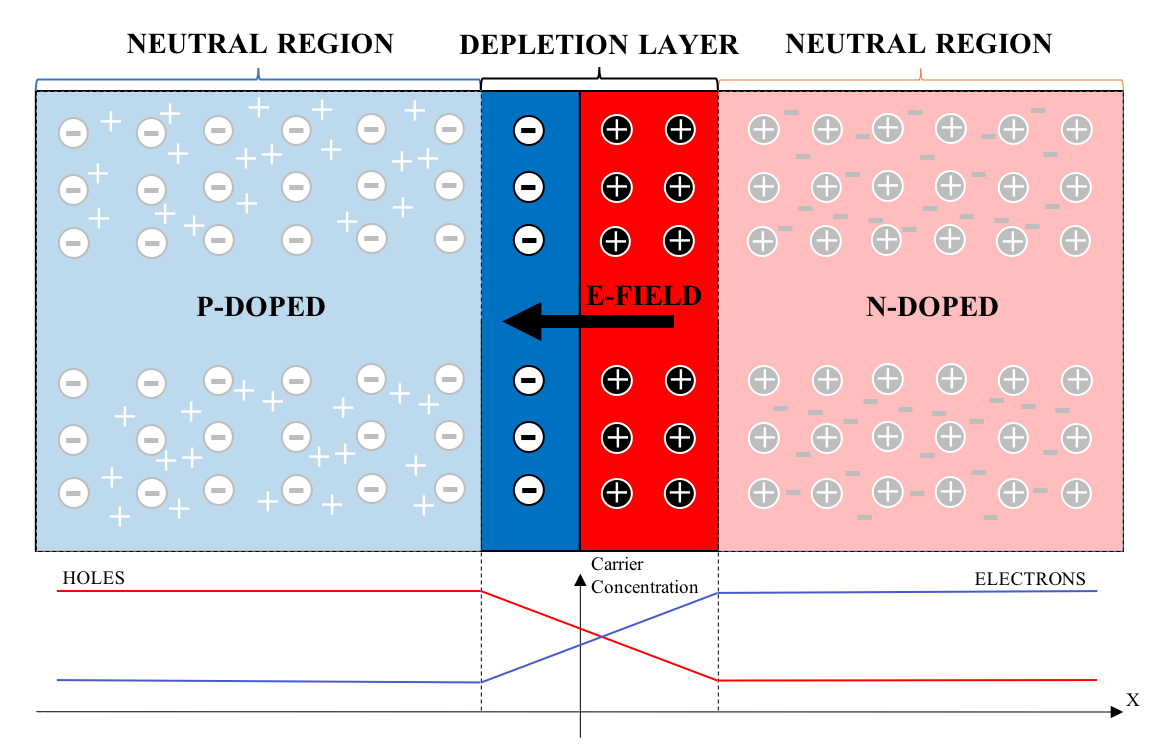
\includegraphics[width=\textwidth]{pn_junction} 
	\caption[A typical illustration of a P-N Junction.]{My own illustration of a P-N Junction, inspired by \textcite{Ghassemi2017}.}
	\label{fig:pn_junction}
\end{figure}

As with all solid state devices, the building blocks of \glspl{sipmt} are P-N Junctions. A p- and n-type material are created by the addition of impurities to a semiconducting material such as silicon. The impurities added to produce the n-type semiconductor increases its number of freely moving electrons, while the impurities added to produce the p-type semiconductor increases its number of freely moving holes. When the two materials are joined, the P-N Junction is formed. As a result of the abundance of charges in each material, a diffusion current forms with electrons moving from the n-type material (leaving behind its immobile positive ions) to combine with the holes in the p-type material. The same occurs vice versa for the excess holes in the p-type material, leaving behind its immobile negative ions. The result is a region adjacent to the junction with no free charges remaining, known as the depletion layer (Figure~\ref{fig:pn_junction}). The charge difference from the immobile ions  produces an electric field inside the depletion layer, that points from its positively charged N side to its negatively charge P side. This electric field opposes the diffusion current and causes an equilibrium to be reached across the junction.

\begin{figure}
	\centering
    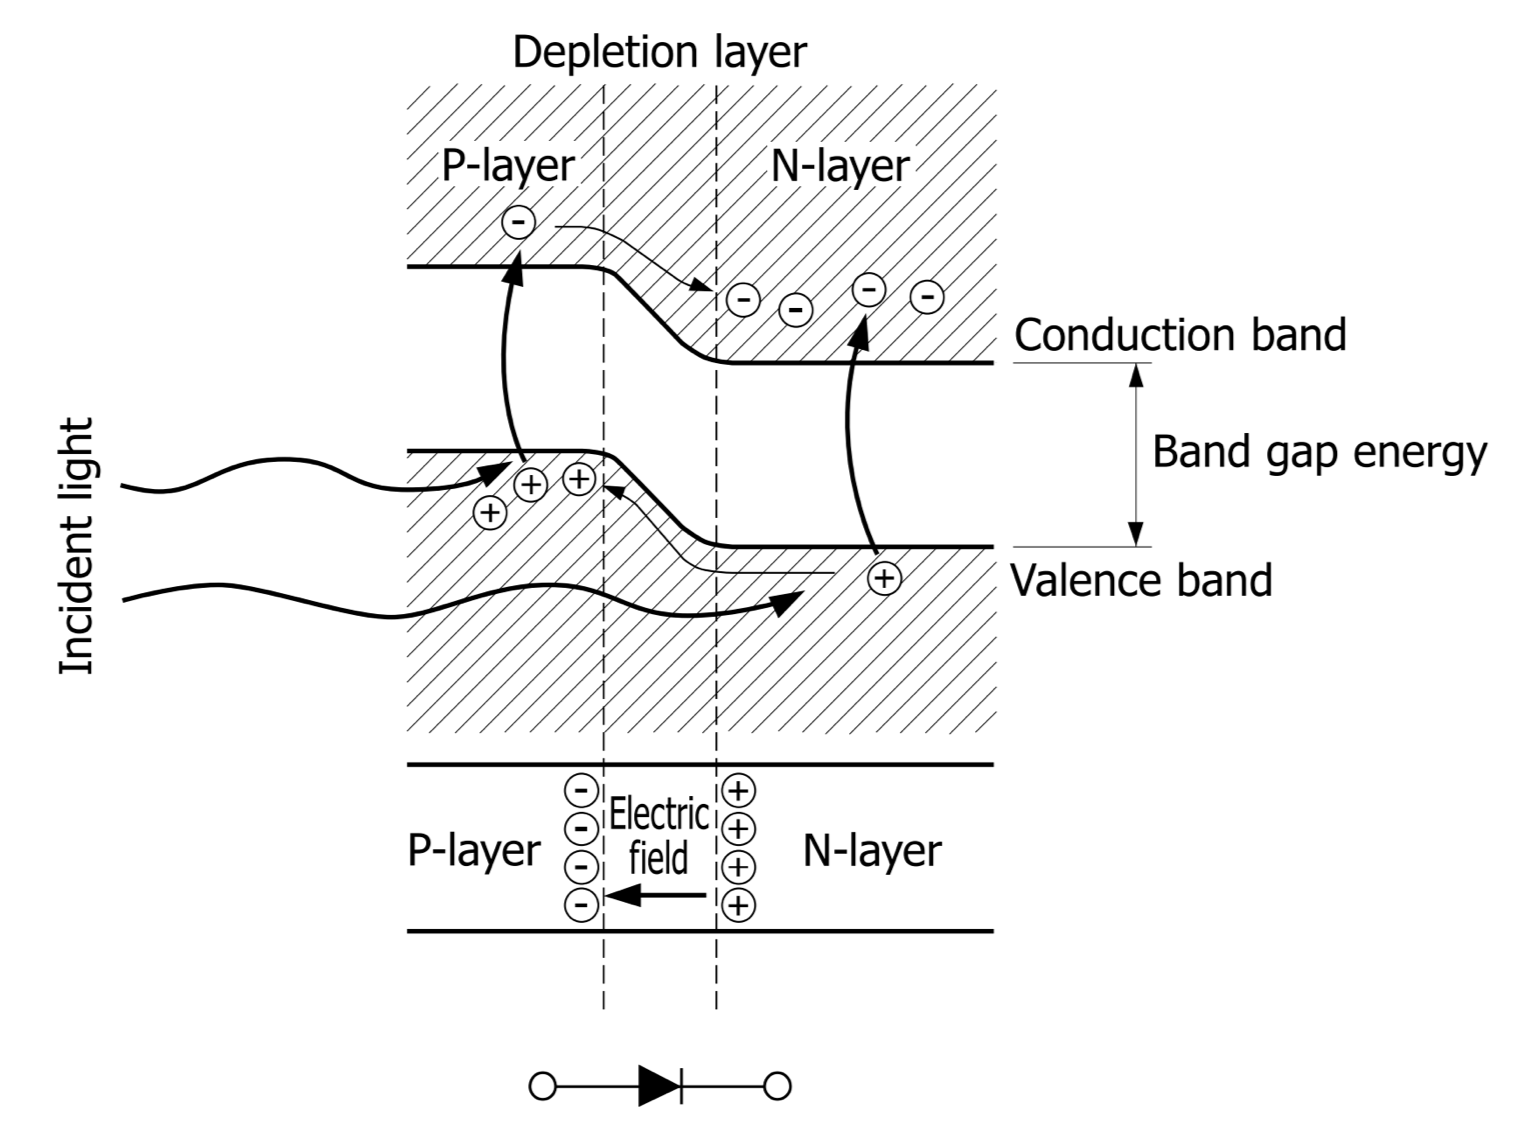
\includegraphics[width=0.6\textwidth]{pn_bandgap} 
	\caption[Illustration of the silicon bandgap.]{Illustration of the silicon bandgap, demonstrating a bound electron being exited into an excess charge carrier via the photoelectric effect. The excess charge carrier is then accelerated in the opposite direction of the electric field, resulting in a current \cite{Ghassemi2017}.}
	\label{fig:pn_bandgap}
\end{figure}

However, this equilibrium can be disturbed by the input of energy into the system, either by thermal excitation (producing what is known as \textit{dark counts}) or by the photoelectric effect. If the energy provided to a bound electron is greater than the band gap energy (inherent to the semiconductor) then it becomes an excess charge carrier, leaving behind a hole. These excess charge carriers are known as an electron-hole pair. If these excess charge carrier are produced in the depletion layer, they will travel along the electric field in the direction according to its charge. For example, an excess electron charge carrier released in the P side of the depletion layer will travel in the opposite direction to the electric field, crossing the P-N Junction to the N side. This is illustrated in Figure~\ref{fig:pn_bandgap}. If a connection is formed between the P and N regions, this process will produce a current. If excess charge carriers are freed outside the depletion layer, they are generally short-lived, as there is no significant electric field to accelerate them, and therefore no net current is produced.

\section{Avalanche PhotoDiode (APD)}

\begin{figure}
	\centering
    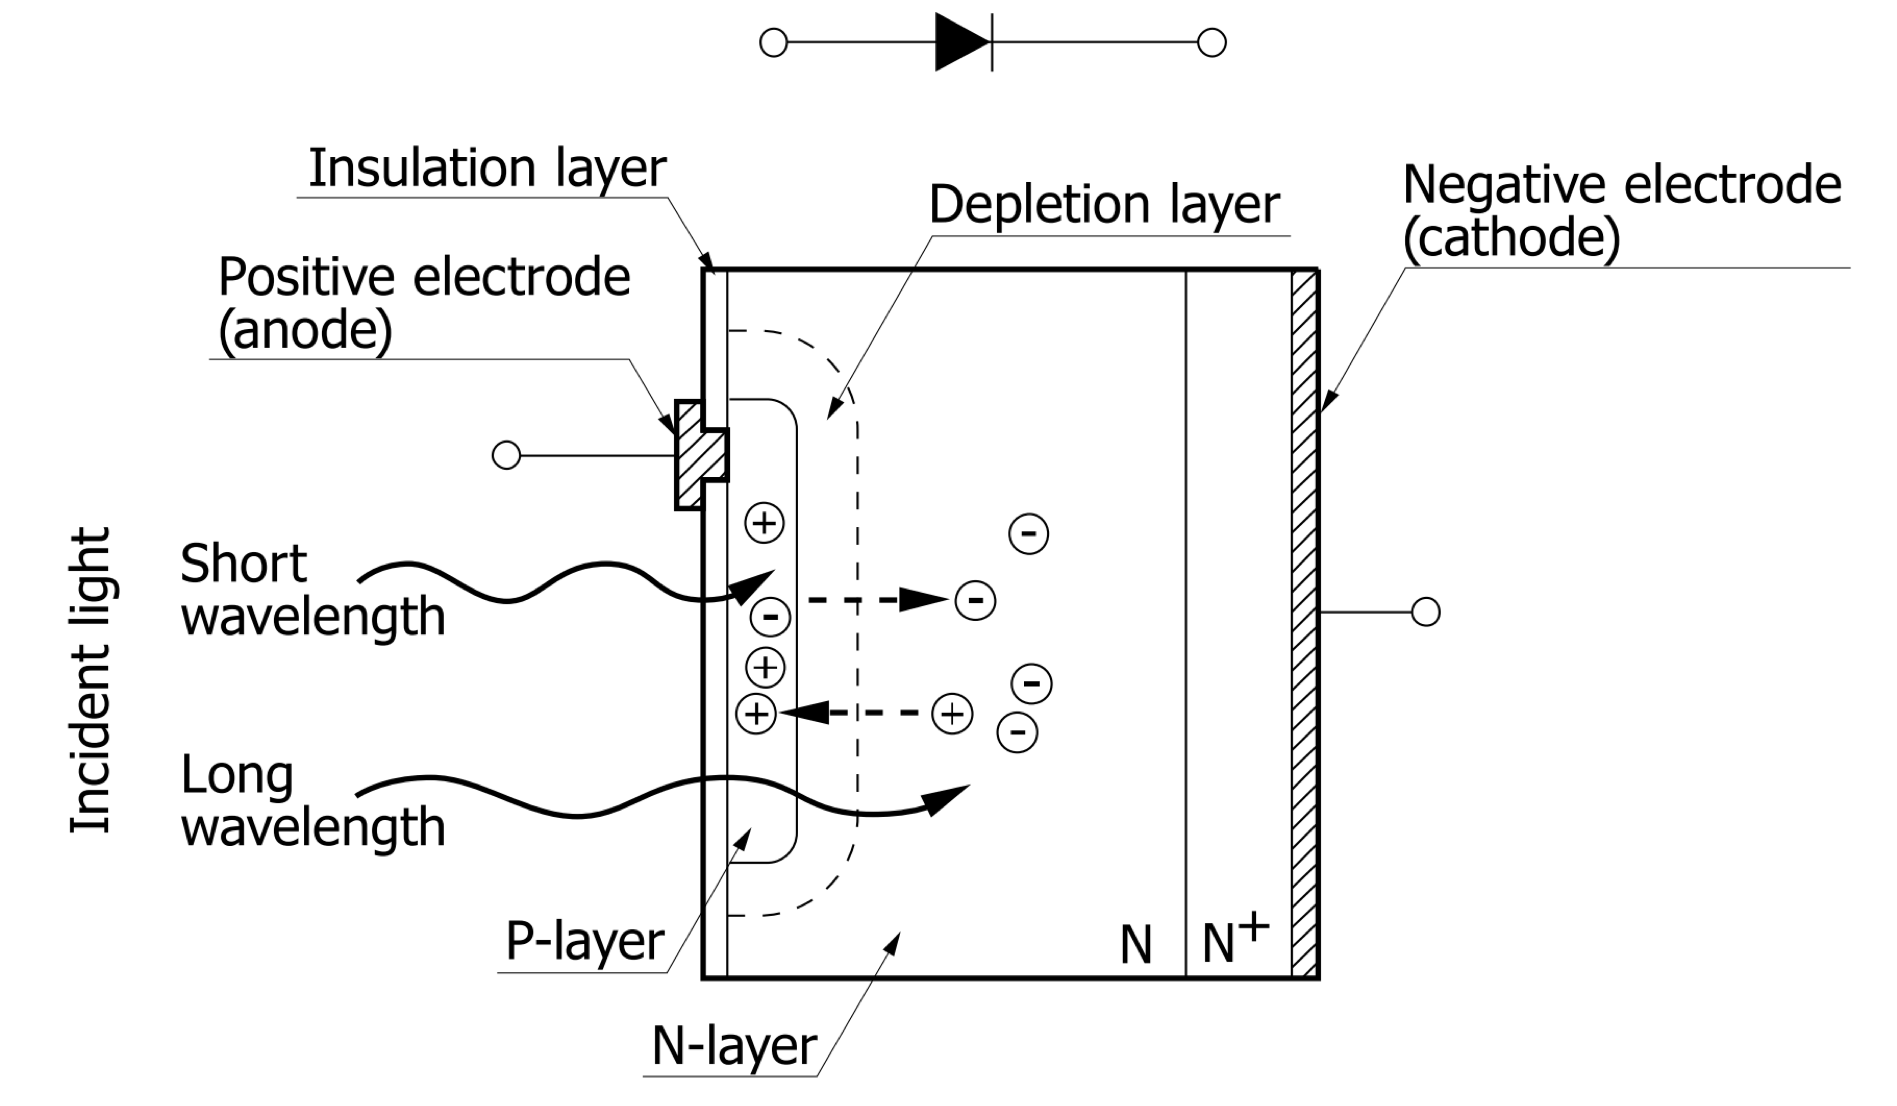
\includegraphics[width=0.6\textwidth]{pn_reversebias} 
	\caption[Diagram of an Avalanche PhotoDiode.]{Diagram of an Avalanche PhotoDiode with a reverse bias voltage applied. The N side of the semiconductor acts as the cathode. Traditionally the cathode is the ``negative electrode'', however in reverse bias the N side is connected to the positive terminal. The P side of the semiconductor acts as the anode. Similarly to the N side, although the anode is the name traditionally given to the ``positive electrode'', in reverse bias the P side is connected to the negative terminal. The result is the electrons are accelerated to the N side cathode, while holes are accelerated to the P side anode \cite{Ghassemi2017}.}
	\label{fig:pn_reversebias}
\end{figure}

In order to maximise the photosensitivity of the semiconductor, the depletion layer depth must be maximised. To achieve this, a reverse bias voltage is applied to the semiconductor. This means biasing the N side (cathode) to a higher electric potential that the P side (anode). The result of this is the freely-mobile holes on the P side, and the freely-mobile electrons on the N side, are pulled away from the junction. This leaves behind the charged ions and causes the depth of the depletion region to increase.

In addition to an increased depletion layer depth, this reverse bias results in an increase in the electric field within the depletion region. Excess charge carriers achieve a higher kinetic energy as a result. If the mean kinetic energy attained between collisions with ions is greater than the band gap energy, additional charge carriers may be released. This impact ionisation effect results in a rapid multiplication of excess charge carriers, and is referred to as an avalanche. Such a device it therefore known as an \gls{apd}. The ratio of final charge carrier signal that is read out to the initial photo-carriers produced is the gain of the \gls{apd}, analogous to the gain of a \gls{pmt}.

The typical operation of a \gls{apd} is to apply the bias voltage that optimally maintains relatively constant bandwidth and stable noise output, while achieving the highest gain level \cite{Ghassemi2017}. This voltage occurs before the \textit{breakdown voltage}, where the gain approach infinity. This operation of the \gls{apd} is known as ``proportional'' or ``linear'' mode \cite{Otte2006}, as the gain increases proportionally with bias voltage. However, \glspl{apd} in this mode suffer from limited gain and large variations in their single amplification, and are therefore not useful in single photon counting. To better utilise \glspl{apd} we must increase the bias voltage beyond the breakdown voltage, causing the \gls{apd} to transition into Geiger mode.

\section{Geiger-mode Avalanche PhotoDiode (G-APD)}

\begin{figure}
	\centering
    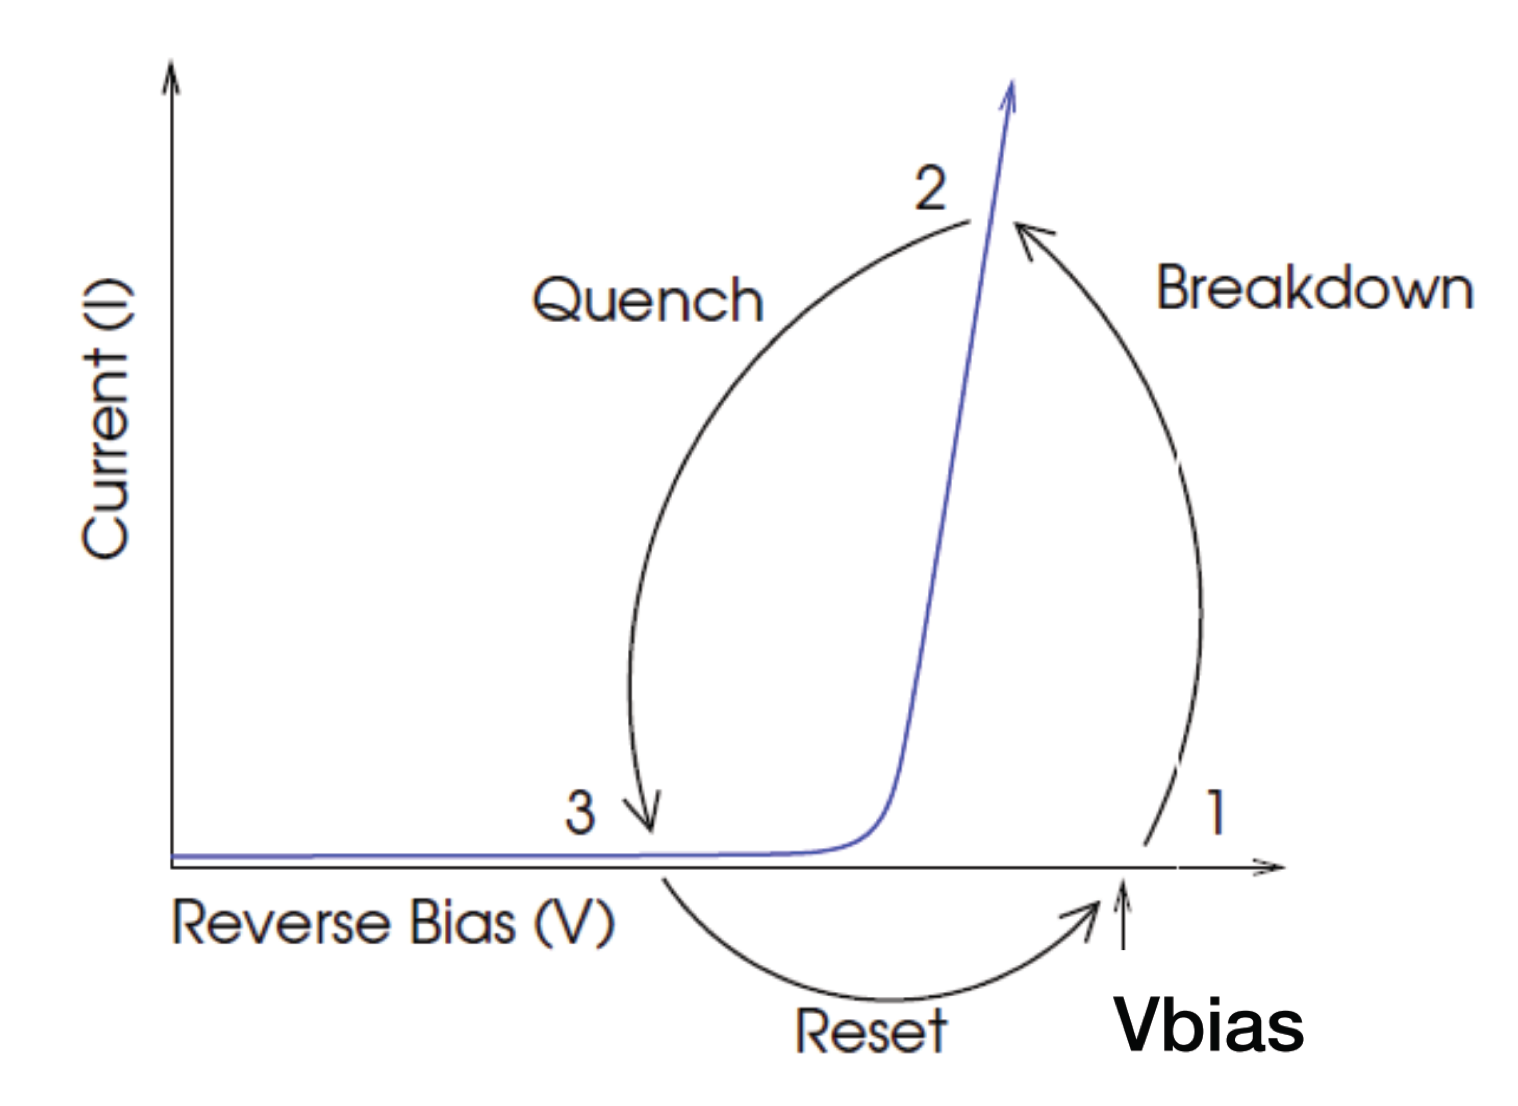
\includegraphics[width=0.6\textwidth]{gapd_cycle} 
	\caption[G-APD reverse bias voltage cycle.]{Diagram of the current created by the avalanche versus reverse bias voltage \cite{SensL2011}. The stages in the cycle of the G-APD operation are labelled. 1) The G-APD is set to a reverse bias voltage above the breakdown voltage. No current flows yet. 2) A excess charge carrier is produced by thermal excitation or the photoelectric effect. The carrier causes a Geiger discharge, creating a macroscopic current. 3) The current is quenched by a resistor in series with the diode. The bias voltage across the diode is reduced below the breakdown voltage, and the avalanche ceases. The G-APD then recharges ready for the next avalanche.}
	\label{fig:gapd_cycle}
\end{figure}

In Geiger mode, a single photoelectron produces a self-perpetuating ionisation cascade. This effectively causes the silicon to become conductive, thereby amplifying the original electron-hole pair into a measurable current flow \cite{SensL2011}. A ``quenching resistor'' is used in series with the diode to limit the current drawn during breakdown, thereby lowering the bias voltage across the diode and bringing it below the breakdown voltage. This halts the avalanche and results in a signal shape that can be read out from the voltage across the quenching resistor. The \gls{sipmt} then undergoes a recovery back to the original ``overvolatage'' above the breakdown voltage, ready for the next photoelectron avalanche. This operation cycle of the \gls{gapd} is shown in Figure~\ref{fig:gapd_cycle}.

The disadvantage of this mode is that the \gls{gapd} is a binary device. All information about the number of generated photoelectrons in the semiconductor is lost. The only knowledge one can have is that there was at least one photoelectron. However, the response that results from this signal, completely independent of the number of initial photoelectrons, is extremely large and well defined, with a gain in the range $10^5$-$10^7$. \glspl{gapd} are therefore very useful as single photon counting devices, but are not so useful in operations where a large dynamic range is desired. 

\section{Silicon Photomultiplier (SiPM)}

\begin{figure}
	\centering
    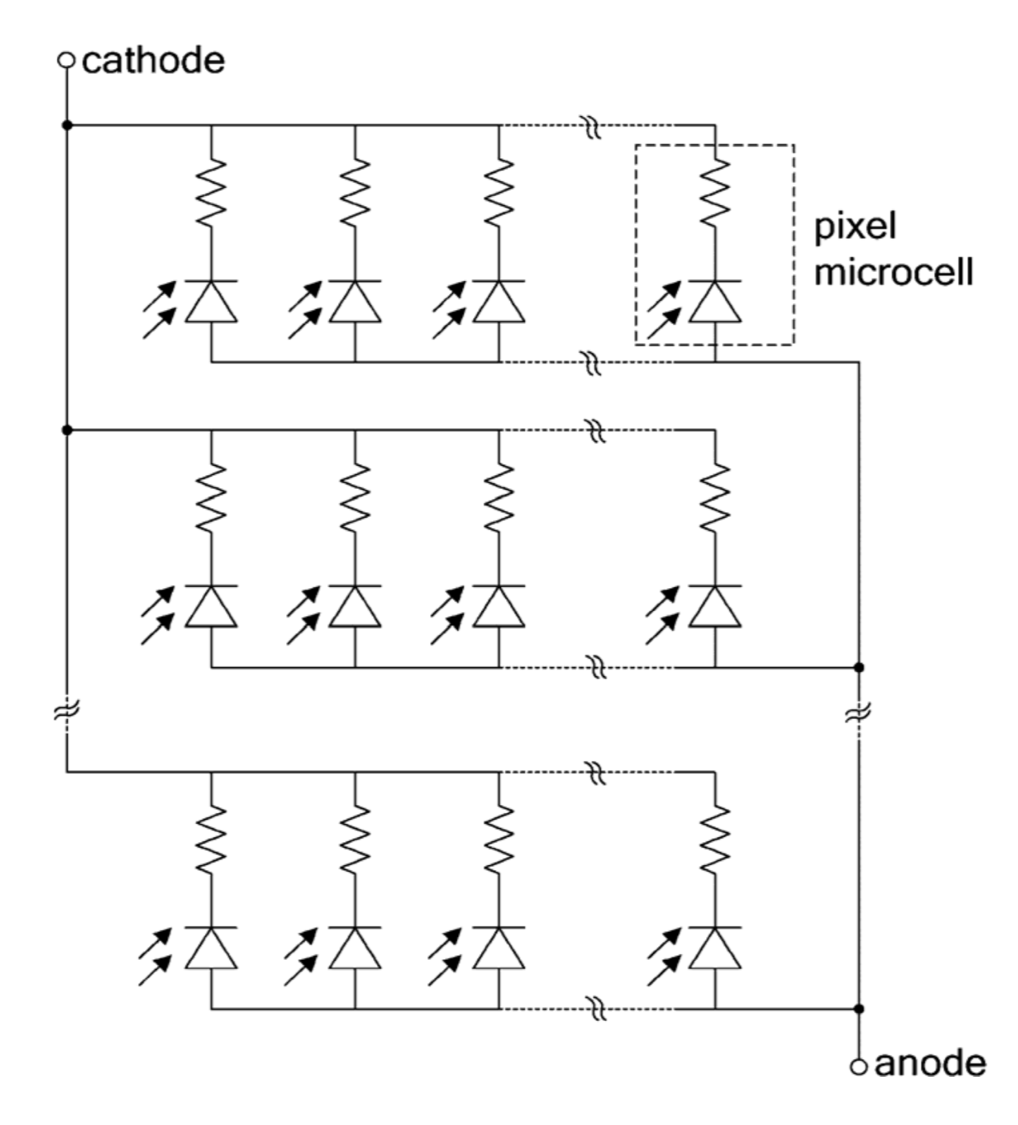
\includegraphics[width=0.6\textwidth]{sipmt_circuit} 
	\caption[Simplified equivalent circuit of an SiPM detector.]{Simplified equivalent circuit of an SiPM detector, demonstrating the individual microcells connected in parallel \cite{Marano2014}.}
	\label{fig:sipmt_circuit}
\end{figure}

The final transition in this technology chain is to the concept of the \gls{sipmt}. This device utilises a densely packed array of up to 10,000 \glspl{gapd} per \si{mm\squared}. Each of these \gls{gapd} ``microcells'' has its own quenching resistor, and all the microcells are connected in parallel to a common bus \cite{Otte2006}. Figure~\ref{fig:sipmt_circuit} shows a simplification of the equivalent circuit diagram for an \gls{sipmt}. The result is a detector that can count multiple photons, with a dynamic range that is essentially the number of microcells. Though, each microcell still operates as a binary sensor, therefore two photons incident on the same cell will only register as one. The superposition of the output current pulses from all the microcells results in the highly quantised measure of the number of photoelectrons produced.